\section{Experimental Results}
To evaluate our work for this paper, we synthesized implementations for 46
Lustre models~\footnote{The models are part of a larger collection
that can be found at
https://tinyurl.com/gt4geqz}~\cite{Hagen08:FMCAD}, including the running example. The original models already contained an implementation,
which provided us with a complete test benchmark suite, since we were able to
compare the synthesized implementations to handwritten programs.

To effectively compare the synthesized programs, we developed a compiler from
primitive scratch files that contain the collection of Skolem functions
describing the implementation, to C programs. We then compared these C
implementations against the original models, after they had been translated
to C using the LustreV6 compiler~\cite{lustrev6}.

\begin{figure}[]
	\centering
	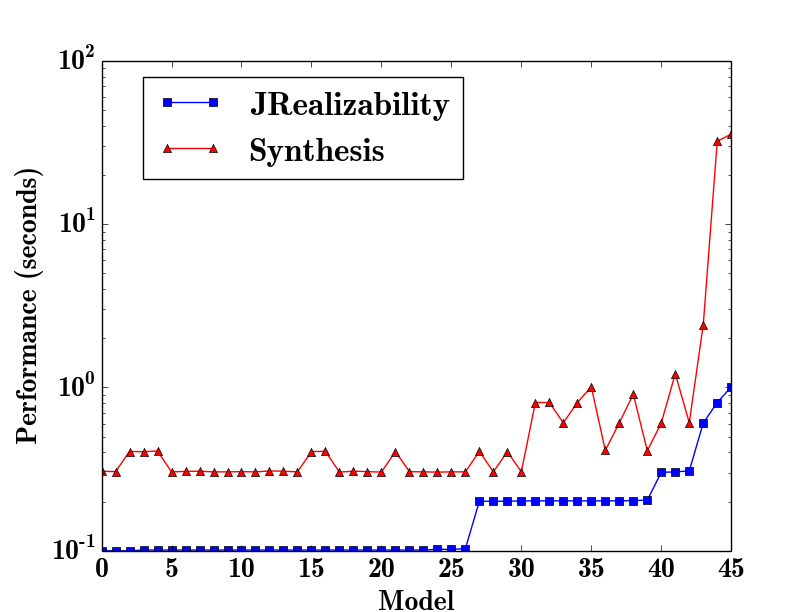
\includegraphics[width=0.8\textwidth,height=\textheight,keepaspectratio]{overhead}    	
	\caption{Overhead of synthesis to realizability checking}
	\label{fg:overhead}
\end{figure}

Figure~\ref{fg:overhead} shows the overhead of our extension to JKind's
realizability checking algorithm to support synthesis. The overhead is at
expected levels for the majority of the models, with a few outstanding
exceptions where it has a significant impact to the overall performance.
A particularly interesting way to improve upon this is by switching to a more
sophisticated algorithm, where we endorse the core idea of Property Directed
Reachability in terms of finding a proof of realizability, in conjunction with
AE-VAL's skolemization procedure.

\begin{figure}[H]
	\centering
	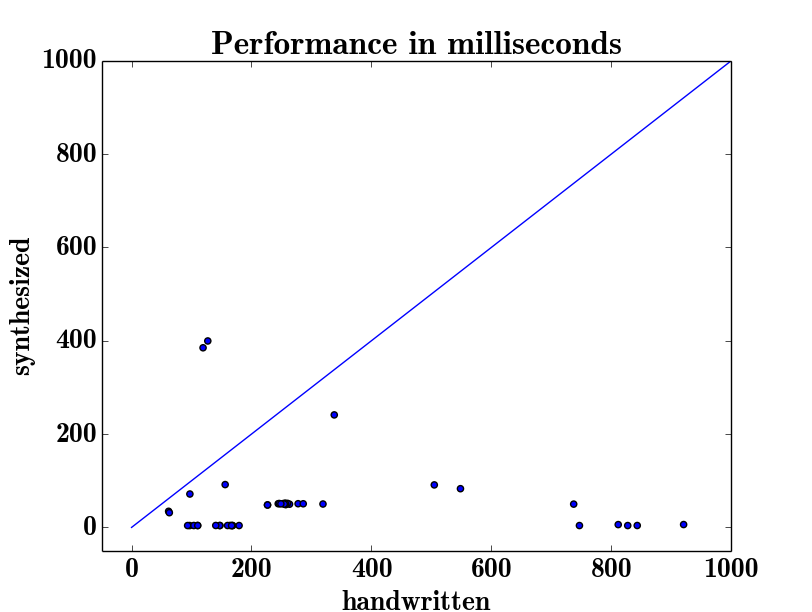
\includegraphics[width=0.8\textwidth,height=\textheight,keepaspectratio]{performance}    	
	\caption{Performance of synthesized and handwritten implementations}
	\label{fg:performance}
\end{figure}

Figure~\ref{fg:performance} provides a scatter plot of the results of our
experiments in terms of the performance of the synthesized programs against the original, handwritten
implementations. Each dot in the scatter plot represents one of the 46
models, with the x axis being the performance of the handwritten
program, while the y axis reports the corresponding performance of the
synthesized implementation. In every case of this benchamrk suite, the
synthesized implementations outperform the programs generated by LustreV6.
We attribute this fact mainly due to the simplicity of the requirements expressed in the files,
as all of them were proved realizable for $k=0$ by JKind, except for the running
example , which was proved for $k=1$.
In addition to the above, we have to take into consideration that LustreV6's C
code generation feature is still documented as work in progress, and thus might
lack optmizations that could possibly help reduce the performance gap.

\begin{figure}[H]
	\centering
	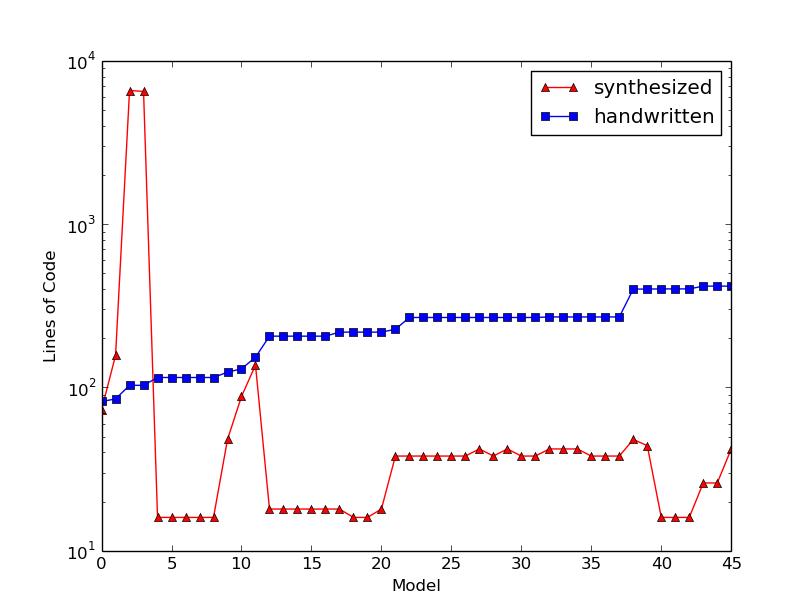
\includegraphics[width=0.8\textwidth,height=\textheight,keepaspectratio]{loc}    	
	\caption{Lines of code of synthesized and handwritten implementations}
	\label{fg:loc}
\end{figure}

Figure~\ref{fg:loc} provides another interesting, as well as important metric in
our experiments, which is the lines of code in each pair of implementations. In
the majority of the models that we used, the overall size of the synthesized
implementation remained well below LustreV6's programs. Despite this, a few
notable outliers still exist, where the actual size of the synthesized
implementation is bigger, with two models exceeding an order of magnitude when
compared to their handwritten counterparts. These two particular models were
also the most complex ones in terms of the specification in our test suite,
and as a result the corresponding Skolem functions are also very big in terms
of size.

For future work, we hope to tackle such cases on three different frontiers. The
first is again the use of a better algorithm that can effectively reduce the size of
the transition relation used during the realizability checking algorithm.
Another interesting idea here is the use of Inductive Validity Cores
(IVCs)~\cite{Ghass16}, whose main purpose is to effectively pinpoint the
absolutely necessary model elements in a generated proof. We can potentially use the
information provided by IVCs as a preprocessing tool to reduce the size of
the original specification, and hopefully the complexity of the realizability
proof. Of course, a few optimizations can be further implemented in terms of
AE-VAL's specific support on proofs of realizability and finally, a very
important subject is the further improvement of the compiler that we created to
translate the Skolem functions into C implementations, by introducing
optimizations like common subexpression elimination.




\label{sec:experiment}
